% Use only LaTeX2e, calling the article.cls class and 12-point type.

\documentclass[12pt]{article}

% Users of the {thebibliography} environment or BibTeX should use the
% scicite.sty package, downloadable from *Science* at
% http://www.sciencemag.org/authors/preparing-manuscripts-using-latex
% This package should properly format in-text
% reference calls and reference-list numbers.

\usepackage{scicite}

\usepackage{times}

\usepackage{subcaption}
\usepackage{graphicx}
\usepackage{floatrow}

% The preamble here sets up a lot of new/revised commands and
% environments.  It's annoying, but please do *not* try to strip these
% out into a separate .sty file (which could lead to the loss of some
% information when we convert the file to other formats).  Instead, keep
% them in the preamble of your main LaTeX source file.


% The following parameters seem to provide a reasonable page setup.

\topmargin 0.0cm
\oddsidemargin 0.2cm
\textwidth 16cm
\textheight 21cm
\footskip 1.0cm


%The next command sets up an environment for the abstract to your paper.

\newenvironment{sciabstract}{%
\begin{quote} \bf}
{\end{quote}}



% Include your paper's title here

\title{The Effectiveness of Strategies to Contain SARS-CoV-2: Testing, Vaccinations, and NPIs}


% Place the author information here.  Please hand-code the contact
% information and notecalls; do *not* use \footnote commands.  Let the
% author contact information appear immediately below the author names
% as shown.  We would also prefer that you don't change the type-size
% settings shown here.

\author
{Janoś Gabler,$^{1, 2}$ Tobias Raabe,$^{3}$ Klara Röhrl,$^{1}$ Hans-Martin von Gaudecker,$^{2,4\ast}$\\
\\
\normalsize{$^{1}$Bonn Graduate School of Economics}\\
\normalsize{$^{2}$IZA Institute of Labor Economics}\\
\normalsize{$^{3}$Private sector}\\
\normalsize{$^{4}$Rheinische Friedrich-Wilhelms-Universität Bonn}\\
\\
\normalsize{$^\ast$To whom correspondence should be addressed; E-mail:  hmgaudecker@uni-bonn.de.}
}

% Include the date command, but leave its argument blank.

\date{}



%%%%%%%%%%%%%%%%% END OF PREAMBLE %%%%%%%%%%%%%%%%



\begin{document}

% Double-space the manuscript.

\baselineskip24pt

% Make the title.

\maketitle



% Place your abstract within the special {sciabstract} environment.

\begin{sciabstract}
    In order to slow the spread of the CoViD-19 pandemic, governments around the world
    have enacted a wide set of policies limiting the transmission of the disease.
    Initially, these focused on non-pharmaceutical interventions; more recently,
    vaccinations and large-scale rapid testing have started to play a major role. The
    objective of this study is to explain the quantitative effects of these policies on
    determining the course of the pandemic, allowing for factors like seasonality or
    virus strains with different transmission profiles. To do so, the study develops an
    agent-based simulation model, which is estimated using data for the second and the
    third wave of the CoViD-19 pandemic in Germany. The paper finds that during a period
    where vaccination rates rose from 5\% to 40\%, seasonality and rapid testing had the
    largest effect on reducing infection numbers. Frequent large-scale rapid testing
    should remain part of strategies to contain CoViD-19; it can substitute for many
    non-pharmaceutical interventions that come at a much larger cost to individuals,
    society, and the economy.
\end{sciabstract}

The development of highly effective vaccines holds the promise of containment in the
medium term. However, most countries find themselves months or years away from reaching
vaccination levels that would end the pandemic \cite{Mathieu2021}. While
non-pharmaceutical interventions (NPIs) have allowed some countries to sustain
equilibria with very low infection numbers \cite{Contreras2021} most have seen large
fluctuations of infection rates over time. It is therefore of utmost importance to
employ an effective mix of strategies for containing the virus. However, the effects of
diverse policies and their interplay with seasonal patterns are not well understood.

This paper develops a quantitative model incorporating these factors simultaneously. The
framework allows to combine a wide variety of data and mechanisms, making it useful to
predict the effects of various interventions. We apply the model to Germany, where new
infections fell by almost 80\% during May 2021. Our analysis shows that, aside from
seasonality, frequent and large-scale rapid testing caused the bulk of this decrease,
which is in line with prior predictions \cite{Mina2021}.

At the core of our agent-based model \cite{Aleta2020,Hinch2020} (we review more
literature in Supplementary Material~Fig.~B.1) are physical contacts
between heterogeneous agents (Figure~\ref{fig:model_contacts_infections}) that
potentially cause infections. Contacts occur in up to four areas: Within the
household, at work, at school, or in other settings. Some contacts recur regularly,
others occur at random. Empirical applications can take the population and household
structure from census data and the network-specific frequencies of contacts from diary
data measuring contacts before the pandemic (e.g. \cite{Mossong2008,Hoang2019}). Within
each network, meeting frequencies depend on age and geographical location (see
Supplementary Material~A.4).

The contact networks are chosen so that the most common NPIs can be modeled in great
detail. NPIs affect the number of contacts or the risk of transmitting the disease upon
having physical contact. NPIs' effects on meeting frequencies will vary across contact
types. Mask mandates or air filters would reduce the probability of infection
\cite{Lessler2021, Cheng2021}. See Supplementary Material~B.4 for
details on how we model NPIs.

\begin{figure}   % Figure 1
    \centering

    \begin{subfigure}[b]{0.425\textwidth}
        \centering
        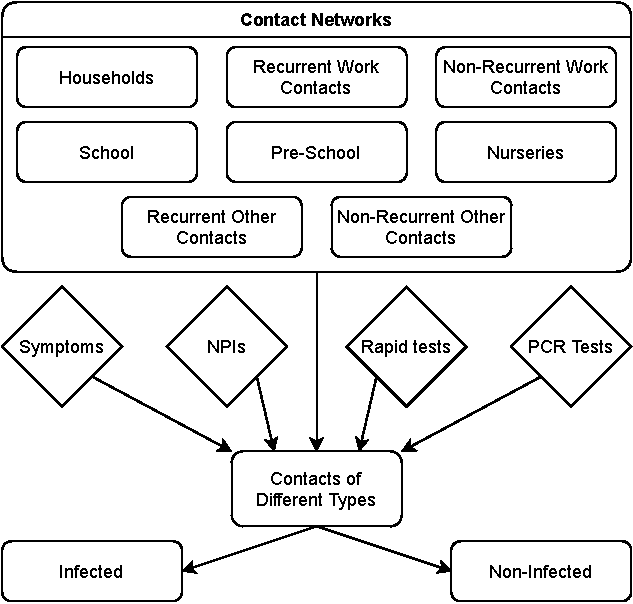
\includegraphics[width=\textwidth]{../figures/model-graph-top-left}
        \caption{{Model for contacts and infections}}
        \label{fig:model_contacts_infections}
    \end{subfigure}
    \hfill
    \begin{subfigure}[b]{0.425\textwidth}
        \centering
        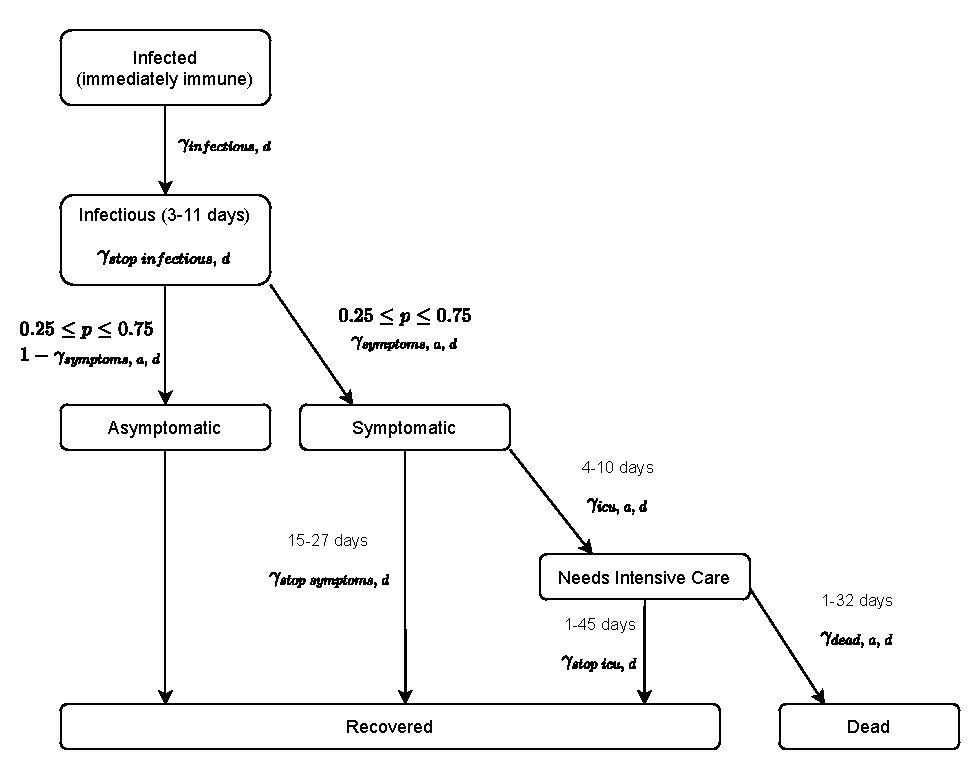
\includegraphics[width=\textwidth]{../figures/model-graph-top-right}
        \vskip5ex

        \caption{Disease progression}
        \label{fig:model_disease_progression}
    \end{subfigure}
    \vskip3ex
    \begin{subfigure}[b]{0.425\textwidth}
        \centering

        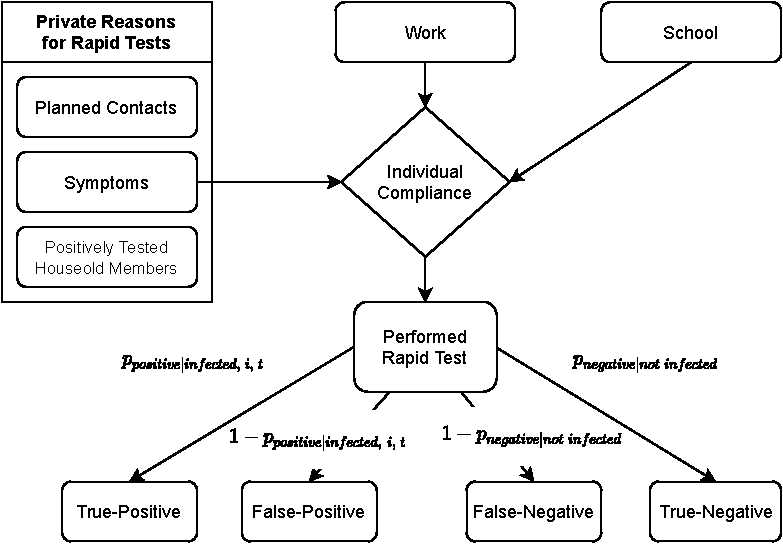
\includegraphics[width=\textwidth]{../figures/model-graph-bottom-left}
        \caption{{Model for rapid tests}}
        \label{fig:model_rapid_tests}
    \end{subfigure}
    \hfill
    \begin{subfigure}[b]{0.425\textwidth}
        \centering
        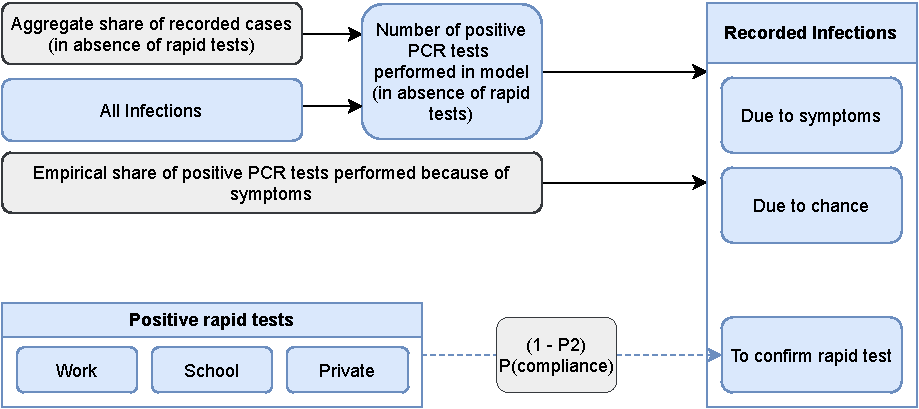
\includegraphics[width=\textwidth]{../figures/model-graph-bottom-right}
        \vskip5ex

        \caption{{Translating all infections to recorded ones}}
        \label{fig:model_official_cases}
    \end{subfigure}

    \caption{Model description}
    \label{fig:model_description}

    \floatfoot{\noindent \textit{Note:}
        A~description of the model can be found in Supplementary Material~B.
        Figure~\ref{fig:model_contacts_infections} shows the influence of an agent's
        contacts to other agents on infections. Demographic characteristics set the
        baseline number of contacts in different networks ($\eta$). The agents may
        reduce the number of contacts due to NPIs, showing symptoms, or testing
        positively for SARS-CoV-2 ($\tau$). Infections may occur when a susceptible
        agent meets an infectious agent; the probability depends on the type of contact
        ($\beta_c$), on seasonality ($\kappa_{c}$), and on NPIs ($\rho_{c,\:t}$). If
        infected, the infection progresses as depicted in
        Figure~\ref{fig:model_disease_progression}. If rapid tests are available,
        agents' demand is modeled as in Figure~\ref{fig:model_rapid_tests}. All reasons
        trigger a test only for a fraction of individuals depending on an individual
        compliance parameter; the thresholds for triggering test demand differ across
        reasons and they may depend on calendar time ($\pi_{c,\:t}$ and $\tau_{c,\:t}$).
        Figure~\ref{fig:model_official_cases} shows the model of translating all
        infections in the simulated data to age-specific recorded infections. The model
        uses data on the aggregate share of recorded cases ($\psi$), the share of
        positive PCR tests triggered by symptoms ($\chi_{symptom}$), and the false
        positive rate of rapid tests ($p_{positive|infected,\;i,\:t}$). The lower part
        of the graph is relevant only for periods where rapid tests are available. All
        parameters are explained in Appendix~A.11.}
\end{figure}

In the model, a possible infection progresses as shown in
Figure~\ref{fig:model_disease_progression} (similar to \cite{Aleta2020}, more in
Supplementary Material~A.1). Whereas susceptibility to the viruses differs by age, the
infectiousness is independent of age conditioned on the type of contact
\cite{Jones2021}.

The model includes several other crucial features. New virus strains with different
infectiousness profiles may appear. Vaccines may become available. During the vaccine
roll-out, priority may depend on age and occupation; vaccine hesitancy is modeled by
some individuals refusing vaccination offers. With some probability, vaccinated agents
become immune and do not transmit the virus \cite{Hunter2021, LevineTiefenbrun2021,
Petter2021, Pritchard2021}.

We include two types of tests. Polymerase chain reaction (PCR) tests reveal with
certainty whether an individual is infected or not; they are scarce and require
at least one day to be processed. In contrast, rapid antigen tests yield
immediate results. Specificity and sensitivity of these tests is set according
to data analyzed in \cite{Bruemmer2021, Smith2021}; sensitivity depends on the
timing of the test relative to the onset of infectiousness (we show our results
are robust to more conservative assumptions in
Section~\ref{subsec:robustness_rapid_test_sensitivity}).
Figure~\ref{fig:model_rapid_tests} shows our model for rapid test demand.
Schools may require staff and students to be tested regularly. Rapid tests may
be offered by employers to on-site workers. Individuals may demand tests for
private reasons, which include having plans to meet other people, showing
symptoms of CoViD-19, and a household member having tested positively for the
virus. We endow each agent with an individual compliance parameter. This
parameter determines whether she takes up rapid tests. Positive tests and
symptoms lead most individuals to reduce their contacts.

Modelling a population of agents according to actual demographic characteristics means
that we can use a wide array of data to identify and calibrate the model's many
parameters (see Supplementary Material~A for a complete description). Examples are
contact diaries, administrative records on case numbers, virus strains, tests and
vaccines as well as surveys on private rapid test demand. Other studies' estimates of
the seasonality of infections can be incorporated directly. The remaining
parameters---most notably, the infection probabilities by contact network and the
effects of some NPIs, see Supplementary Material~A.9---will be chosen numerically so
that the model matches features of the data (see \cite{McFadden1989} for the general
method). By modelling PCR and rapid tests in detail, we can translate infection numbers
in the model into observed infections before matching them to the data. The mechanism is
depicted in Figure~\ref{fig:model_official_cases} and described in Supplementary
Material~B.7. Figure~B.9 shows the resulting share of detected cases.

The model is applied to the second and third waves of infections in Germany, covering
the period September 2020 to May 2021. Figure~\ref{fig:pandemic_drivers_model_fit}
describes the evolution of the pandemic and of its drivers. The black line in
Figure~\ref{fig:aggregated_fit} shows officially recorded cases; the black line in
Figure~\ref{fig:stringency_infectious_contacts} a rescaled Oxford Response Stringency
Index \cite{Hale2020}, which tracks the tightness of non-pharmaceutical interventions.
Between mid September and early November, cases increased tenfold. Restrictions were
somewhat tightened in mid-October and again in early November. New infections remained
constant throughout November before rising again in December, prompting the most
stringent lockdown to this date. Schools and daycare centers were closed, so were
customer-facing businesses except for grocery and drug stores. From the peak of the
second wave just before Christmas until the trough in mid-February, newly detected cases
decreased by almost three quarters. The third wave in the spring of 2021 is associated
with the B.1.1.7 (Alpha) strain, which became dominant in March
(Figure~\ref{fig:share_b117}). In early March, some NPIs were relaxed. There were many
changes in details of regulations afterwards, but they did not change the overall
stringency index.

\begin{figure}[!tp]   % Figure 2
    \centering

    \begin{subfigure}[b]{0.475\textwidth}
        \centering
        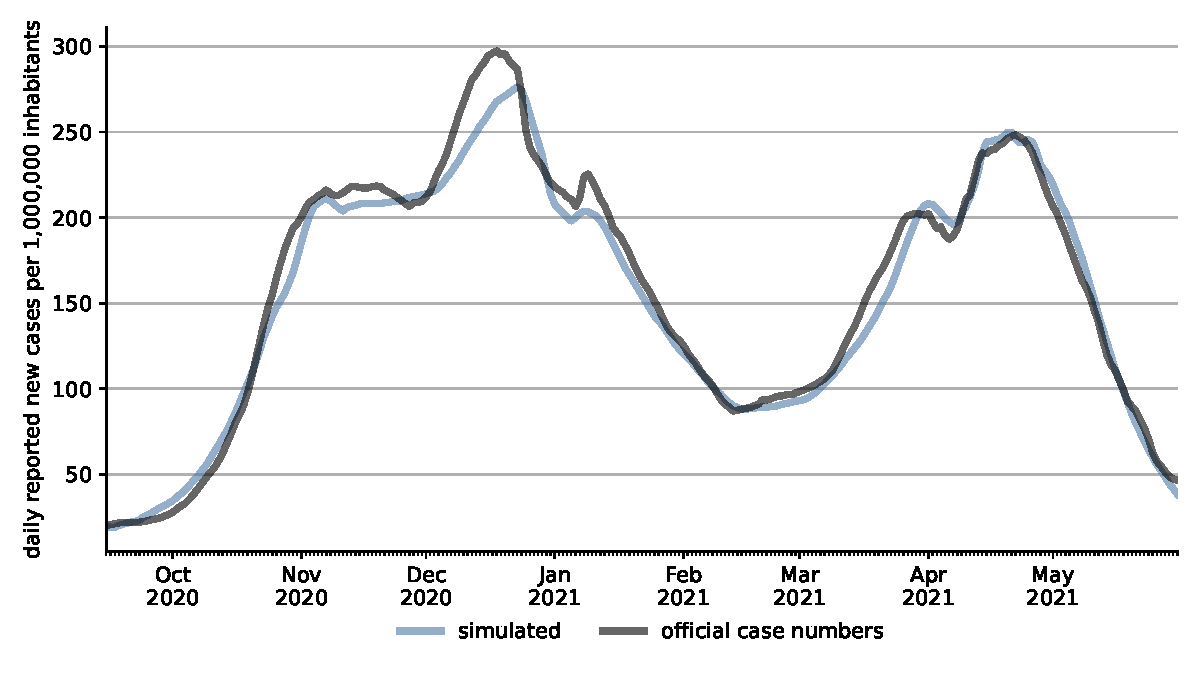
\includegraphics[width=\textwidth]{../figures/results/figures/scenario_comparisons/combined_fit/full_new_known_case}
        \caption{{Recorded cases: Empirical and simulated}}
        \label{fig:aggregated_fit}
    \end{subfigure}
    \hfill
    \begin{subfigure}[b]{0.475\textwidth}
        \centering
        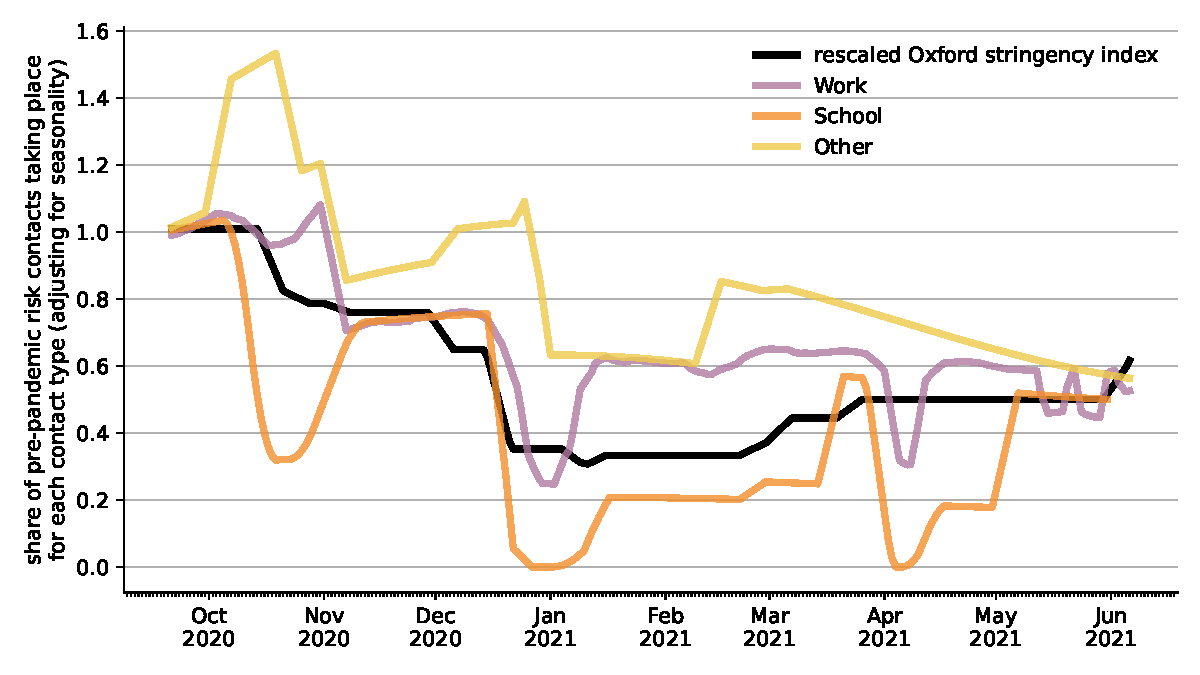
\includegraphics[width=\textwidth]{../figures/results/figures/data/stringency2_with_seasonality}

        \caption{{Stringency of NPIs and infectious contacts}}
        \label{fig:stringency_infectious_contacts}
    \end{subfigure}

    \vskip3ex

    \begin{subfigure}[b]{0.475\textwidth}
        \centering

        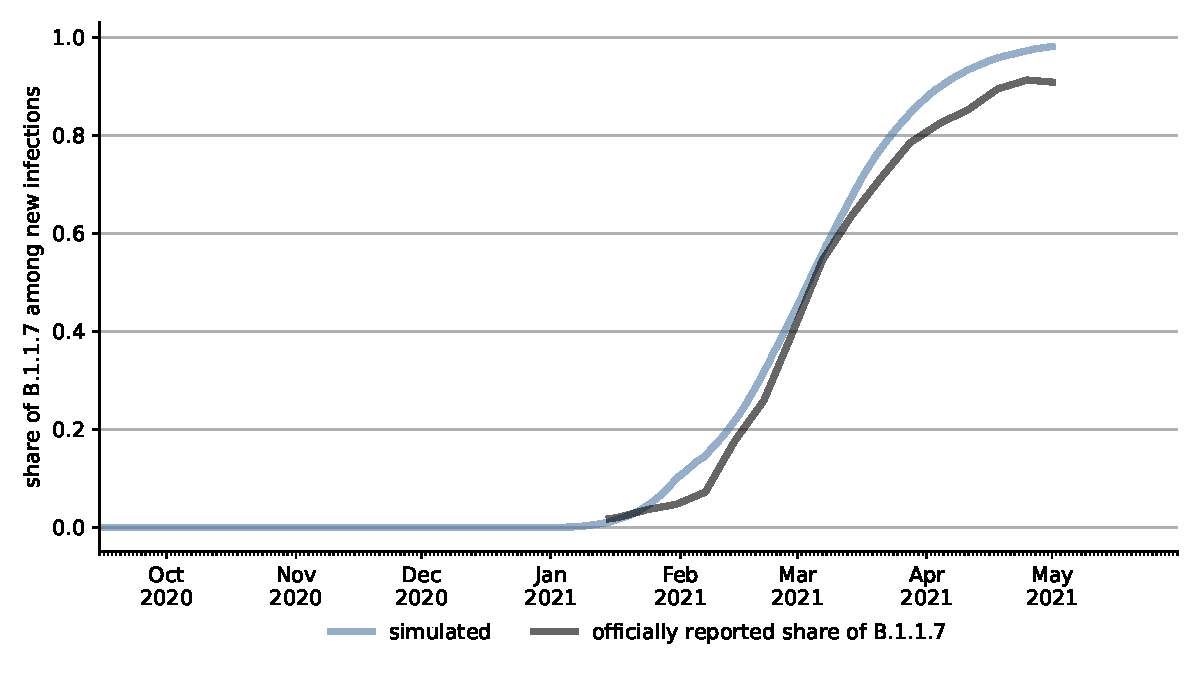
\includegraphics[width=\textwidth]{../figures/results/figures/scenario_comparisons/combined_fit/full_share_b117}

        \caption{Fraction of B.1.1.7 strain}
        \label{fig:share_b117}
    \end{subfigure}
    \hfill
    \begin{subfigure}[b]{0.475\textwidth}
        \centering

        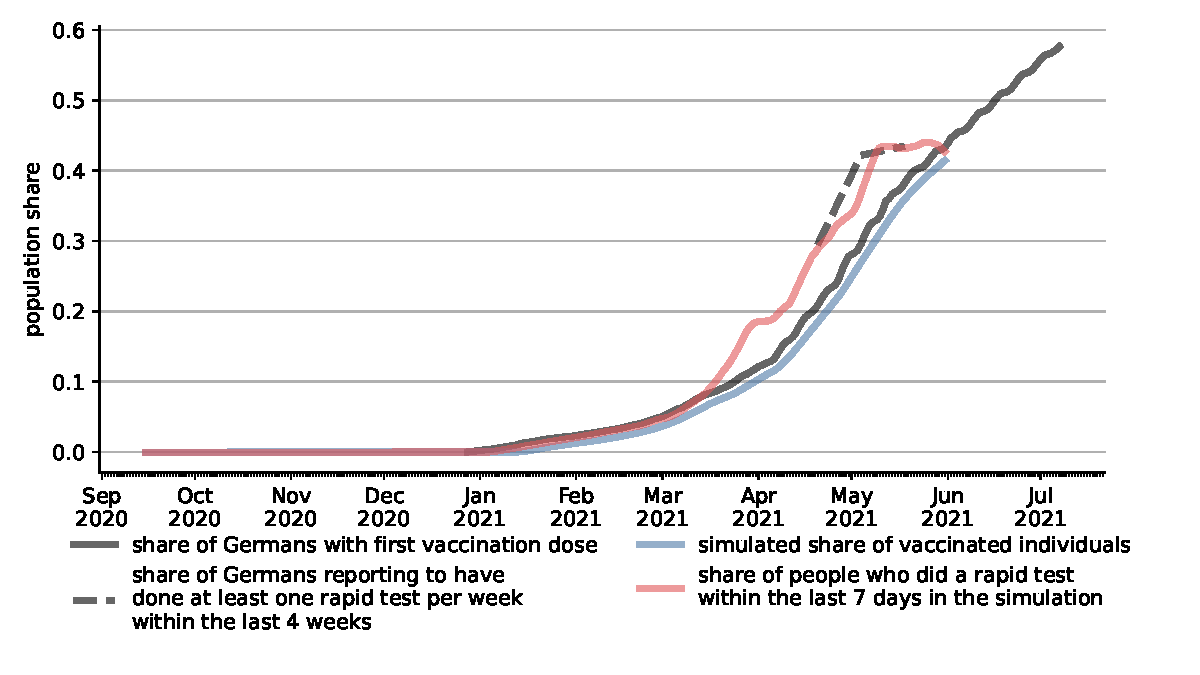
\includegraphics[width=\textwidth]{../figures/results/figures/scenario_comparisons/combined_fit/full_share_rapid_test_in_last_week_and_vaccinated}

        \caption{{Tests and vaccinations}}
        \label{fig:antigen_tests_vaccinations}
    \end{subfigure}

    \caption{Evolution of the pandemic, its drivers, and model fit, September 2020 to May 2021}
    \label{fig:pandemic_drivers_model_fit}

    \floatfoot{\noindent \textit{Note:} Data sources are described in Supplementary
        Material~A. Age- and region-specific analogues to
        Figure~\ref{fig:aggregated_fit} can be found in Supplementary Material B.10. For
        legibility reasons, all lines in Figure~\ref{fig:stringency_infectious_contacts}
        are rolling 7-day averages. The Oxford Response Stringency Index is scaled as $2
        \cdot (1 -  x / 100)$, so that a value of one refers to the situation at the
        start of our sample period and zero means that all NPIs included in the index
        are turned on. The other lines in
        Figure~\ref{fig:stringency_infectious_contacts} show the product of the effect
        of contact reductions, increased hygiene regulations, and seasonality. See
        Appendix~A.5 for separate plots of the three factors by contact type.}
\end{figure}

Around the turn of the year, the first people were vaccinated with a focus on older age
groups and medical staff (Figure~\ref{fig:antigen_tests_vaccinations}). Until the end of
May, 43\% had received at least one dose of a vaccine. In late 2020, rapid tests started
to replace regular PCR tests for staff in many medical and nursing facilities. At-home
tests approved by authorities became available in mid-March. Rapid test centers were
opened, and one test per person and week was made available free of charge. In several
states, customers were only allowed to enter certain stores with a recent negative rapid
test result. These developments are characteristic of many countries: The initial focus
on NPIs to slow the spread of the disease has been accompanied by vaccines and a growing
acceptance and use of rapid tests.

We draw simulated samples of agents from the population structure in September 2020 and
use the model to predict recorded infection rates until May 2021. See Supplementary
Materials~A.2 and B.9 for details. The blue line in Figure~\ref{fig:aggregated_fit}
shows that our model's predictions are very close to officially recorded cases in the
aggregate. This is also true for infections by age and geographical region (see
Supplementary Material~B.10).

The effects of various mechanisms can be disentangled due to the distinct temporal
variation in the drivers of the pandemic. Next to the stringency index, the three lines
in Figure~\ref{fig:stringency_infectious_contacts} summarize how contact reductions,
increased hygiene regulations, and seasonality evolved since early September for each of
the three broad contact networks. For example, a value of 0.75 for the work multiplier
means that if the environment was the same as in September (levels of infection rates,
no rapid tests or vaccinations, only the wildtype virus present), infections at the
workplace would be reduced by 25\%. Two aspects are particularly interesting. First, all
lines broadly follow the stringency index and they would do so even more if we left out
seasonality and school vacations. Second, the most stringent regulations coincide with
the period of decreasing infection rates between late December 2020 and mid-February
2021. The subsequent reversal of the trend is associated with the spread of the B.1.1.7
variant. During the steep drop in recorded cases during May 2021, for 42\% of the
population took at least one rapid tests per week, the first-dose vaccination rate rose
from 28\% to 43\%, and seasonality lowered the relative infectiousness of contacts.

In order to better understand the contributions of rapid tests, vaccinations, and
seasonality on the evolution of infections, Figure~\ref{fig:2021_scenarios_broad}
considers various scenarios. NPIs are always held constant at their values in the
baseline scenario. Figure~\ref{fig:2021_scenarios_recorded} shows the model fit (the
blue line, same as in Figure~\ref{fig:aggregated_fit}), a scenario without any of the
three factors (red line), and three scenarios turning each of these factors on
individually. Figure~\ref{fig:2021_scenarios_newly_infected} does the same for total
infections in the model. Figure~\ref{fig:2021_scenarios_decomposition} employs Shapley
values \cite{Shapley2016} to decompose the difference in total infections between the
scenario without any of the three factors and our main specification.

\begin{figure}[!tp]
    \centering

    \begin{subfigure}[b]{0.475\textwidth}
        \centering
        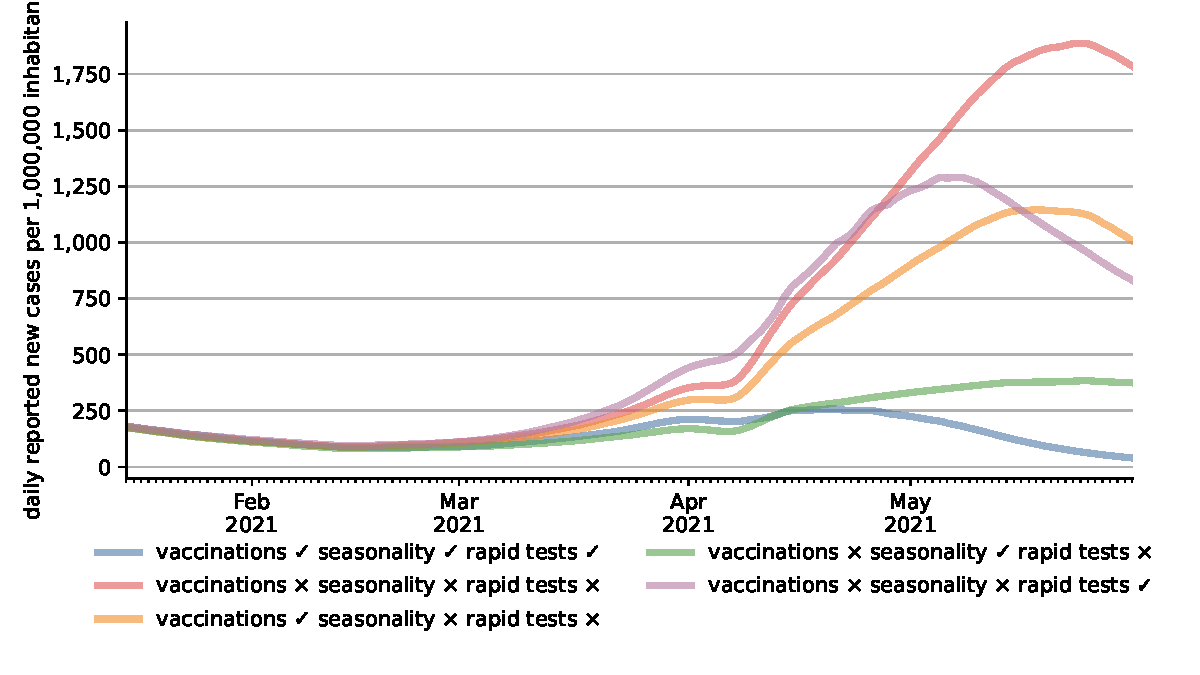
\includegraphics[width=\textwidth]{../figures/results/figures/scenario_comparisons/effect_of_channels_on_pessimistic_scenario/full_new_known_case}
        \caption{{Recorded cases: 2021 scenarios}}
        \label{fig:2021_scenarios_recorded}
    \end{subfigure}
    \hfill
    \begin{subfigure}[b]{0.475\textwidth}
        \centering
        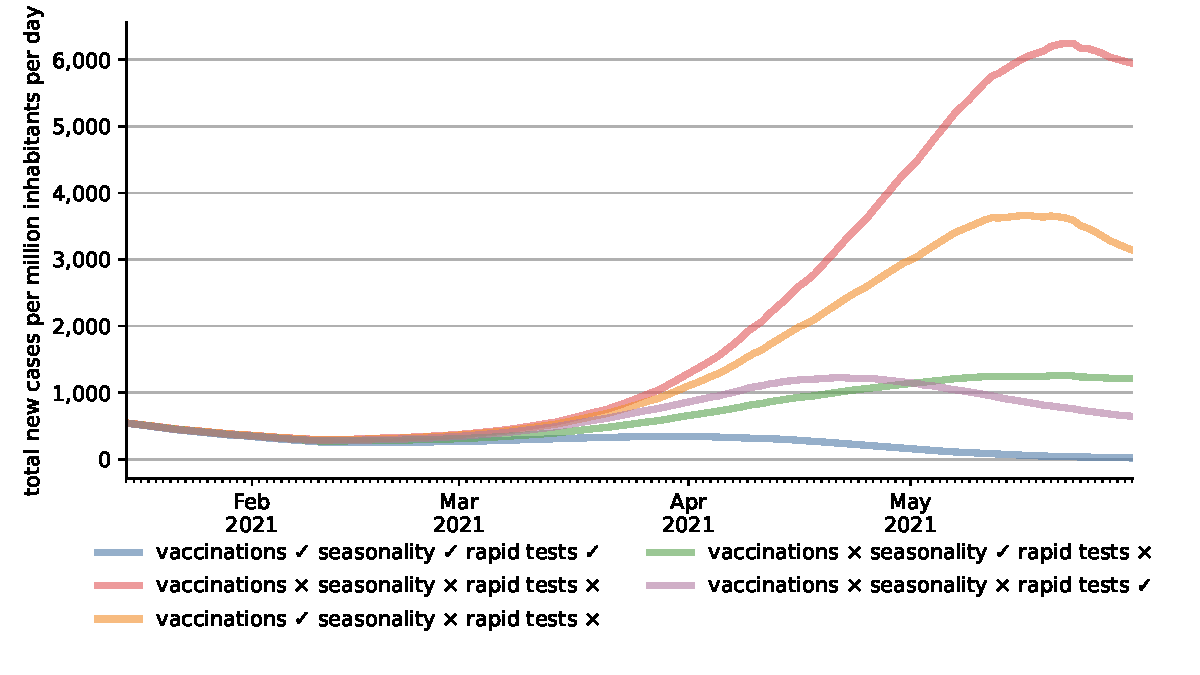
\includegraphics[width=\textwidth]{../figures/results/figures/scenario_comparisons/effect_of_channels_on_pessimistic_scenario/full_newly_infected}
        \caption{{Total cases: 2021 scenarios}}
        \label{fig:2021_scenarios_newly_infected}
    \end{subfigure}

    \begin{subfigure}[b]{0.475\textwidth}
        \centering
        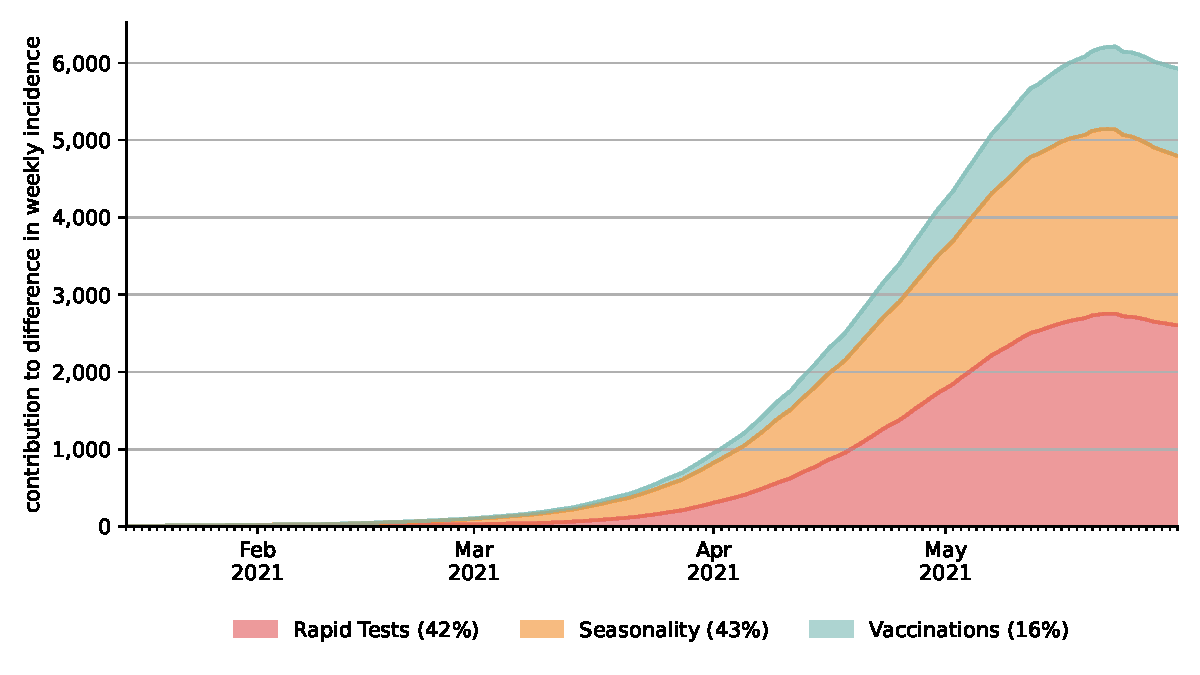
\includegraphics[width=\textwidth]{../figures/results/figures/full_decomposition_channels_area}
        \caption{Decomposition of the difference between the scenario without any of the
            three factors and the main scenario in
            Figure~\ref{fig:2021_scenarios_newly_infected}.}
        \label{fig:2021_scenarios_decomposition}
    \end{subfigure}
    \hfill
    \begin{subfigure}[b]{0.475\textwidth}
        \centering
        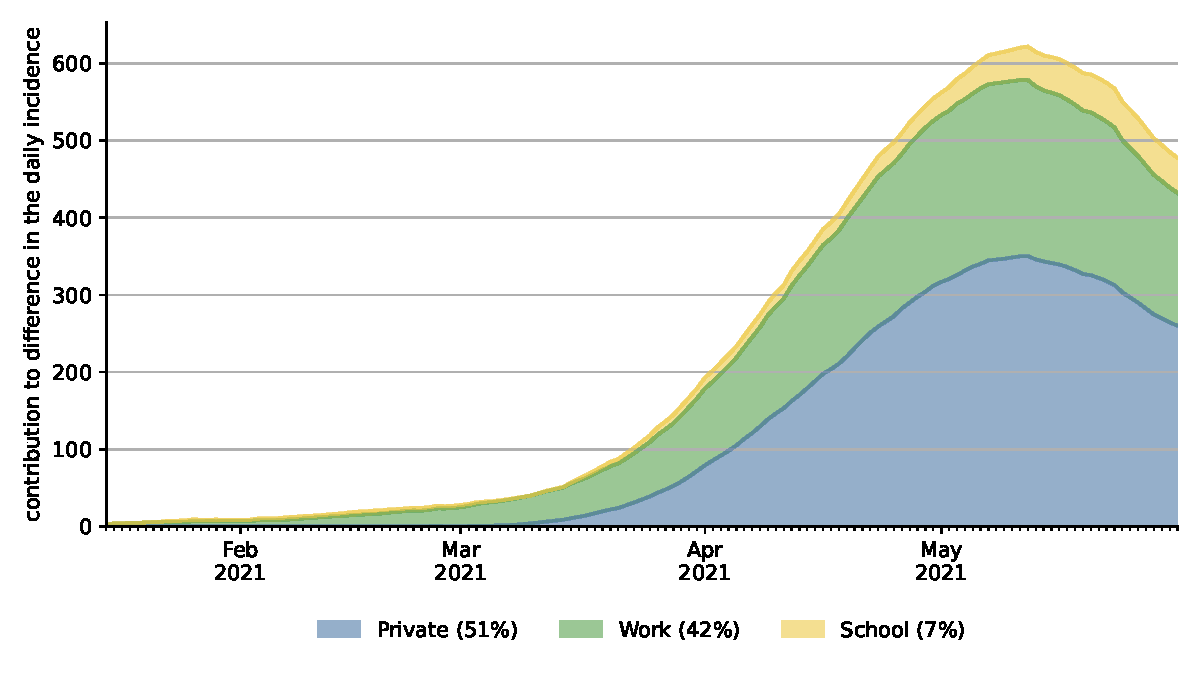
\includegraphics[width=\textwidth]{../figures/results/figures/full_decomposition_rapid_tests_area}
        \caption{Decomposition of the difference between the scenario without rapid
            tests and the main scenario in
            Figure~\ref{fig:2021_scenarios_newly_infected}.}
        \label{fig:2021_scenarios_decomposition_tests}
    \end{subfigure}

    \caption{The effect of different interventions on recorded and actual infections}
    \label{fig:2021_scenarios_broad}

    \floatfoot{\noindent \textit{Note:} The blue line in
        Figure~\ref{fig:2021_scenarios_recorded} is the same as in
        Figure~\ref{fig:aggregated_fit} and refers to our baseline scenario, so does the
        blue line in Figure~\ref{fig:2021_scenarios_newly_infected}. The red lines refer
        to a situation where NPIs evolve as in the baseline scenario and the B.1.1.7
        variant is introduced in the same way; vaccinations, rapid tests, and
        seasonality remain at their January levels. The other scenarios turn each of
        these three factors on individually. The decompositions in
        Figures~\ref{fig:2021_scenarios_decomposition} and
        \ref{fig:2021_scenarios_decomposition_tests} are based on Shapley values, which
        are explained in Appendix~A.10. All lines are rolling 7-day averages.
    }
\end{figure}

Until mid-March, there is no visible difference between the different scenarios. Even
thereafter, the effect of the vaccination campaign is surprisingly small. The Shapley
value decomposition shows that vaccinations contribute 16\% to the cumulative difference
between scenarios. Reasons for the low share are the slow start and the focus on older
individuals who typically have fewer contacts. By the end of our study period, when
first-dose vaccination rates reached 43\% of the population, the numbers of new cases
would have started to decline.

Seasonality has a large effect in slowing the spread of SARS-CoV-2. By May 31, both
observed and total cases would be reduced by a factor of four if only seasonality
mattered. However, in this period, cases would have kept on rising throughout, just at a
much lower pace (this is in line with results in \cite{Gavenciak2021}, which our
seasonality measure is based on). Nevertheless, we estimate seasonality to be an
important factor, explaining most of the early changes and 43\% of the cumulative
difference by the end of May.

A similar-sized effect---42\% in the decomposition---comes from rapid testing. Here, it
is crucial to differentiate between recorded cases and actual cases. Additional testing
means that additional infections will be recorded which would otherwise remain
undetected. Figure~\ref{fig:2021_scenarios_recorded} shows that this effect is large and
may persist for some time. Until late April, recorded cases are higher in the scenario
with rapid testing alone when compared to the setting where none of the three mechanisms
are turned on. The effect on total cases, however, is visible immediately in
Figure~\ref{fig:2021_scenarios_newly_infected}.

So why is rapid testing so effective? In order to shed more light on this question,
Figure~\ref{fig:2021_scenarios_decomposition_tests} decomposes the difference in the
scenario without rapid tests and the main specification into the three channels for
rapid tests. Tests at schools have the smallest effect, which is largely explained by
schools not operating at full capacity during our period of study and the relatively
small number of students.\footnote{18\% of our population are in the education sector
(pupils, teachers, etc.); 46\% are workers outside the education sector.} Almost 40\%
come from tests at the workplace. Despite the fact that rapid tests for private reasons
are phased in only in mid-March, they make up for more than half of the total effect.
The reason lies in the fact that a substantial share of these tests is driven by an
elevated probability to carry the virus, i.e., showing symptoms of CoViD-19 or following
up on a positive test of a household member. This is essentially a form of contact
tracing, which has been shown to be very effective \cite{Contreras2021,
Fetzer2021,Kretzschmar2020}. Indeed, a deeper analysis in Supplementary Material~B.14
shows that the same amount of rapid tests administered randomly in the population would
not have been nearly as effective. Furthermore, mandating tests at schools almost
offsets the increased infection risk of opening schools (see Figure~B.13a).

Our analysis has shown that during the transition to high levels of vaccination and
possibly thereafter, large-scale rapid testing can substitute for some NPIs. This comes
at a fraction of the cost. A day of strict lockdown is estimated to have cost around
50~Euros per capita \cite{Dorn2020b}; retail prices for rapid tests were below one Euro
in early June 2021. Widespread availability of self-administered tests at low prices are
likely to play a role for indication-driven testing. Mandatory tests in schools and at
the workplace are important to screen the entire population, also because disadvantaged
groups are less likely to be reached by testing campaigns relying on voluntary
participation (e.g. \cite{StillmanTonin2021}); at the same time, these groups have a
higher risk to contract CoViD-19 \cite{KochInstitut2021a}. Compared to vaccinations,
rapid testing programmes allow a much quicker roll-out, making it arguably the most
effective tool to contain the pandemic in the short run.

% \bibliography{bibliography}
% \bibliographystyle{Science}

\begin{thebibliography}{10}

\bibitem{Mathieu2021}
E.~Mathieu, {\it et~al.\/}, {\it Nature Human Behaviour\/}  (2021).

\bibitem{Contreras2021}
S.~Contreras, {\it et~al.\/}, {\it arXiv\/}  (2021).

\bibitem{Mina2021}
M.~J. Mina, K.~G. Andersen, {\it Science\/} {\bf 371}, 126 (2021).

\bibitem{Aleta2020}
A.~Aleta, {\it et~al.\/}, {\it Nature Human Behaviour\/} {\bf 4}, 964 (2020).

\bibitem{Hinch2020}
R.~Hinch, {\it et~al.\/}, {\it medRxiv\/}  (2020).

\bibitem{Mossong2008}
J.~Mossong, {\it et~al.\/}, {\it PLoS medicine\/} {\bf 5} (2008).

\bibitem{Hoang2019}
T.~Hoang, {\it et~al.\/}, {\it Epidemiology\/} {\bf 30}, 723 (2019).

\bibitem{Lessler2021}
J.~Lessler, {\it et~al.\/}, {\it Science\/} {\bf 372}, 1092 (2021).

\bibitem{Cheng2021}
Y.~Cheng, {\it et~al.\/}, {\it Science\/}  (2021).

\bibitem{Jones2021}
T.~C. Jones, {\it et~al.\/}, {\it Science\/}  (2021).

\bibitem{Hunter2021}
P.~R. Hunter, J.~Brainard, {\it medRxiv\/}  (2021).

\bibitem{LevineTiefenbrun2021}
M.~Levine-Tiefenbrun, {\it et~al.\/}, {\it Nature medicine\/} {\bf 27}, 790
  (2021).

\bibitem{Petter2021}
E.~Petter, {\it et~al.\/}, {\it medRxiv\/}  (2021).

\bibitem{Pritchard2021}
E.~Pritchard, {\it et~al.\/} .

\bibitem{Bruemmer2021}
L.~E. Br\"{u}mmer, {\it et~al.\/}, {\it medRxiv\/}  (2021).

\bibitem{Smith2021}
R.~L. Smith, {\it et~al.\/}, {\it The Journal of Infectious Diseases\/}
  (2021). Jiab337.

\bibitem{McFadden1989}
D.~McFadden, {\it Econometrica: Journal of the Econometric Society\/} pp.
  995--1026 (1989).

\bibitem{Hale2020}
T.~Hale, {\it et~al.\/}, {\it Blavatnik School of Government\/}  (2020).

\bibitem{Shapley2016}
L.~S. Shapley, {\it 17. A value for n-person games\/} (Princeton University
  Press, 2016).

\bibitem{Gavenciak2021}
T.~Gaven{\v c}iak, {\it et~al.\/}, {\it medRxiv\/}  (2021).

\bibitem{Fetzer2021}
T.~Fetzer, T.~Graeber, {\it Forthcoming, Proceedings of the National Academy of
  Sciences\/}  (2021).

\bibitem{Kretzschmar2020}
M.~E. Kretzschmar, {\it et~al.\/}, {\it The Lancet Public Health\/} {\bf 5},
  e452 (2020).

\bibitem{Dorn2020b}
F.~Dorn, {\it et~al.\/}, {\it ifo Schnelldienst\/} {\bf 73}, 29 (2020).

\bibitem{StillmanTonin2021}
S.~Stillman, M.~Tonin, Communities and testing for {COVID-19} (2021). IZA
  Discussion Paper No. 14012.

\bibitem{KochInstitut2021a}
{Robert Koch-Institut}, Corona-monitoring bundesweit (rki-soep-studie), {\it
  Tech. rep.\/}, {Robert Koch-Institut} (2021).

\end{thebibliography}


\section*{Acknowledgments}

The authors are grateful for support by the Deutsche Forschungsgemeinschaft (DFG, German
Research Foundation) under Germany´s Excellence Strategy – EXC 2126/1– 390838866 – and
through CRC-TR 224 (Projects A02 and C01), by the IZA Institute of Labor Economics, and
by the Google Cloud CoViD-19 research credits program.

\section*{Ethical declarations}

\subsection*{Competing interests}

The authors declare no competing interests.

%Here you should list the contents of your Supplementary Materials -- below is an
%example. You should include a list of Supplementary figures, Tables, and any references
%that appear only in the SM. Note that the reference numbering continues from the main
%text to the SM. In the example below, Refs. 4-10 were cited only in the SM.

\section*{Supplementary materials}

Appendix A - Materials and Methods\\
Appendix B - Supplementary Text\\
Figs. A.1-A.10, B.1-B.16\\
Tables A.1-A.6\\
References \textit{(26-111)}

\end{document}
